\newpage
\chapter{Софтуерна архитектура}
\label{chapter03}

Разработката на софтуер е в областта на инженерните науки, тъй като продуктът се създава по принципите за изграждане на конструкции (в случая софтуерни). При стартирането на нов софтуерен проект трябва да се вземат редица решения според заданието на потребителя. Цел на настоящото помагало е софтуерно решение, което извършва изчисления от страната на клиентски мобилни устройства. Задачите за пресмятане се възлагат от сървър и получените пресметнати резултати се получават обратно на същата машина. От страната на клиента се получават стойности за цена на валути под формата на времеви ред. Сървърът изпраща на клиента също информацията за топология на изкуствена невронна мрежа. Клиентът, от своя страна, използва котировките на валутите и информацията, за изкуствената невронна мрежа за да извършва пресмятанията, необходими за обучението на изкуствената невронна мрежа. Процесът по обучението на изкуствената невронна мрежа\index{изкуствени невронни мрежи} се извършва с помощта на генетични алгоритми\index{генетични алгоритми}, които имат за цел търсене на възможно по-близки до оптималните стойности за теглата на мрежата. Клиентското приложение също поема отговорностите за {\color{red} визуализация} на процеса по обучение и визуализация на постигнатите прогнози. Така представенаq системата съвсем естествено води към избора на  софтуерна архитектура  „клиент-сървър“. 

\section{Избор на развойни средства}

В съвременната софтуерна индустрия има голям избор от развойни средства\index{развойни средства} за различните нужди на софтуерните разработчици. Една част от развойните средства са комерсиални, докато друга част са инструменти с отворен код. В настоящото помагало, акцентът основно пада върху развойни средства с отворен код, тъй като минимизирането на разходите за производство е основен стремеж с цел постигане на икономическа ефективност. Изборът на развойни инструменти е задача от областта на многокритериалния анализ и основно се характеризира с наличието на множество критерии, които често са противоречиви. 

\subsection{От страна на сървъра}

За уеб базирани сървър решения най-популярни са технологиите JSP, ASP, PHP и Node.js. Тъй като ASP е комерсиална технология на фирмата Microsoft тя не представлява интерес за настоящото помагало. JSP e технология на фирмата Oracle която е с отворен код и дава възможност за изграждане на стабилни корпоративни решения. Недостатък на JSP е нуждата от по-сериозни софтуерни и хардуерни ресурси по отношение на хостинга. Node.js е технология, която набира все по-голяма популярност, но все още не е достигнала достатъчно ниво на „зрялост“ като същевременно също изисква повече софтуерни и хардуерни ресурси от страна на хостинга. По отношение на PHP, технологията е с тясно предназначение и има едно от най-високите нива на „зрялост“. В същото време, разходите за хостинг при PHP са едни от най-ниските, което прави изборът на тази технология изключително икономически ефективен. Задачата на уеб базираната сървър технология е да служи като посредник между мрежата и системата за управление на бази от данните. От страна на сървъра най-рационално е данните да се съхраняват в релационна база данни. Съществуват множество решения, които да бъдат приложени в тази част на системата като най-популярните са: Oracle, MS SQL Server, PostgreSQL и MySQL. Oracle намира своето приложение в корпоративния сегмент и е свързан със значителни финансови разходи, което го прави неприемлив за настоящото помагало. MS SQL Server е алтернативна система  на Oracle в корпоративния сегмент и също е свързана със значителни финансови разходи. PostgreSQL е система с отворен код, която е съизмерима с технологичните възможности на Oracle и е потенциално добър кандидат за ниско бюджетни разработки. В настоящото помагало PostgreSQL е избегнат поради своята ненужна сложност, при едно относително просто софтуерно решение. Изборът пада върху MySQL, тъй като системата е максимално опростена добре наложена сред потребителите и се поддържа от фирмата Oracle. Освен всичко изброено, MySQL има добра поддръжка при хостинг доставчиците и е икономически най-ефективният избор. 

\subsection{От страна на клиента}

При „умните“ мобилни устройства най-разпространените операционни системи са Android, iOS и Windows Phone. По настоящем фирмата Microsoft преустанови развитието на своята операционна система Windows Phone, което моментално води до отхвърлянето й за настоящото разглеждане. Инвестицията за разработка на приложения под iOS на фирмата Apple води до отпадането на тази платформа за нуждите на настоящото помагало. Към разходите за разработка може да се добави и фактът, че програмирането за iOS се извършва на два езика Objective-C и Swift, които имат относително малка популярност в Източна Европа. Най-много „умни“ мобилни устройства в световен мащаб се използват с операционната система Android. Android е с отворен код, поддържа се основно от компанията Google и позволява разработка със значително по-ниски финансови разходи, спрямо конкурентите си. Приложенията за Android основно се разработват на езика Java, който по настоящем е един от най-широко използваните програмни езици и се характеризира с много висока степен на „зрялост“. 

\subsection{За комуникация между сървъра и клиента}

Съществуват множество възможности за изграждането на комуникацията между сървъра и клиента. В най-суров вид информацията може да се предава като серия байтове (plane text), което води до множество затруднения при получаването и последващата й обработка. Широко използвана алтернатива е тагиращият език XML. При този вариант информацията бива „пакетирана“ в серия от тагове, които дават определена структура и семантика. Основният замисъл при проектирането на XML е бил създаването на структурирани документи както от хора, така и от машини. Поради тази причина XML има една по-голяма експресивност в сравнение с неговата алтернатива JSON. JSON е максимално опростен тагиращ език за структурирано представяне на информацията, който води своето начало от обектите в програмния език JavaScript. За разлика от XML, JSON има основно предназначение за обмяна на структурирана информация между машини, а не толкова между хора и машини. Поради всичко изброено, в настоящото помагало изборът пада върху JSON като основа за изграждането на комуникационния протокол между сървъра и неговите клиенти. Тъй като от страната на сървъра се предвижда уеб базирано решение, то JSON базираният протокол ще протича в комуникационни сесии на HTTP протокола. В зората на уеб страниците е разработен протоколът HTTP, стъпващ на TCP/IP, за ефективно предаване на информация между уеб сървърите и уеб браузърите. HTTP протоколът е добре наложен и с добра поддръжка в световен мащаб. Една важна негова характеристика е, че при този протокол комуникацията е разделена на заявки и отговори без да се поддържа постоянна комуникационна линия. 

\section{Компоненти на системата}

След направения кратък обзор на технологии и развойни средства изборът е за създаването на „клиент-сървър“ система. От страна на сървъра се разполагат модули за съхранение на данните (MySQL система за управление на бази от данни) и за комуникация (PHP уеб скриптове). Уеб сървърът комуникира с клиентите на база JSON/HTTP комуникационен протокол. Android мобилни устройства правят уеб заявки, извършват изчисленията и връщат резултата до сървъра. Тъй като се разчита на дарена изчислителна мощност\index{дарени изчислителни ресурси}, е нужно да се избере подходящ начин за използване на мобилното устройство без това да нарушава основните му функции и без да пречи на потребителите. Със своята технология Active Wallpaper, Android предлага идеална възможност за целите на настоящото помагало. Активният тапет представлява изображение, което се изрисува зад всички основни графични компоненти от графичния потребителски интерфейс на Android. По-същественото е, че активният тапет е Java приложение, което работи в постоянен фонов режим и може да изпълнява определени кратки задачи, когато устройството не е високо натоварено. 

\begin{figure}[h]
  \centering
  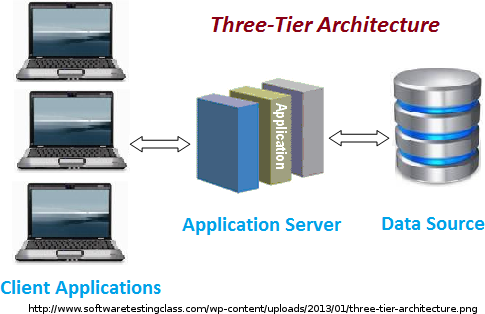
\includegraphics[height=0.25\pdfpageheight]{pic0008}
  \caption{Уеб базирана трислойна софтуерна архитектура}
\label{fig:pic0008}
\end{figure}

При реализацията на настоящата система за изчисления в разпределена среда\index{изчисления в разпределена среда}, изборът пада върху класическа трислойна софтуерна архитектура. Същият подход за три слоя се прилага и при реализацията на мобилното приложение, където SQLite локално съхранява данните над които се работи, Java обектно-ориентиран код извършва изчисленията, а Android базиран графичен потребителски интерфейс поема отговорността за визуализацията на процеса пред потребителя. 

\subsection{Подход за разработка}

\begin{figure}[h]
  \centering
  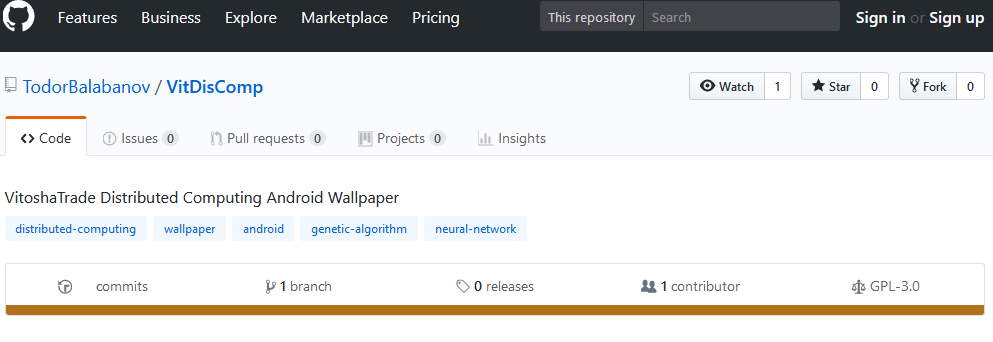
\includegraphics[width=1.0\linewidth]{pic0009}
  \caption{Подходи за софтуерна разработка}
\label{fig:pic0009}
\end{figure}

Ако приемем, че визуализацията е най-горният слой, а базата данни най-долният слой на една трислойна софтуерна архитектура, то има два основни подхода за изработване на софтуерната система (Фиг. \ref{fig:pic0009}). При първия подход първоначално се разработва визуалния интерфейс, след това слоя на работната логика и накрая базата данни. Този подход се нарича „top-down“ и е полезен, когато се анализира софтуерно задание, при което вече има в употреба множество хартиени документи (първоизточници на работните екрани. Този подход също е удобен при проекти с малък размер, където базата данни е относително опростена. Вторият много популярен подход е когато се започне с проектирането на базата данни, след това работната логика, която обработва данните и едва накрая екраните, визуализиращи информацията. Този подход се нарича „bottom-up“ и е най-подходящ, когато се разработва сложно софтуерно решение, което се очаква да работи с големи обеми данни и множество различни структури на информацията. Акцентът в настоящото помагало е върху изчисленията които мобилните устройства извършват, а не толкова към създаването на голям масив от данни. Поради тази причина изборът в случая пада върху подхода „top-down“. 

\section{Лиценз и хранилище за проекта}

При съвременните софтуерни проекти с отворен код са от значение две неща – юридическият лиценз\index{софтуерни лицензи} под който съществува проектът и публичното хранилище\index{хранилища за програмен код}, в което е разположен програмният текст. 

\subsection{Лиценз}

От съществено значение е изборът на правилен софтуерен лиценз, когато се разработва софтуерен проект предвиден да бъде публично достъпен. Съществуват множество възможности като някои от най-популярните са - BSD License, MIT license, Mozilla Public License и GNU General Public License. За нуждите на настоящото помагало е предпочетен GNU General Public License v3, защото този лиценз е най-предпазващ за създателя на софтуерния продукт. В най-общи линии GPL3 позволява - комерсиална употреба, модификации, разпространение, включване в патенти и употреба за лични нужди. Лицензът съпровожда изключително ограничена отговорност за създателите на продукта и абсолютно никаква гаранция за употребата му от страна на потребителите. Лицензът също налага и серия ограничения – задължително включване на текст за авторските права на създателите, списък на извършените промени, не позволява закриване на кода и задължава всяко надграждане на продукта да бъде под същия лиценз. Със своята протекционистка природа GPL е един от лицензите дал най-силен тласък в развитието на продукти с отворен код, което е достатъчна причина да бъде избран за разработки без ясно изразена комерсиална насоченост. 

\subsection{Хранилище за програмен код}

Прието е всеки проект да има название, което особено важи в света на софтуера с отворен код. За настоящото помагало е избрано името VitDisComp. Това название е избрано, тъй като разработката ще се възползва от наличното сървър решение в проекта VIToshatrade \cite{vtrade} и по своята същност проектът е DIStributed COMPuting решение. 

\begin{figure}[h]
  \centering
  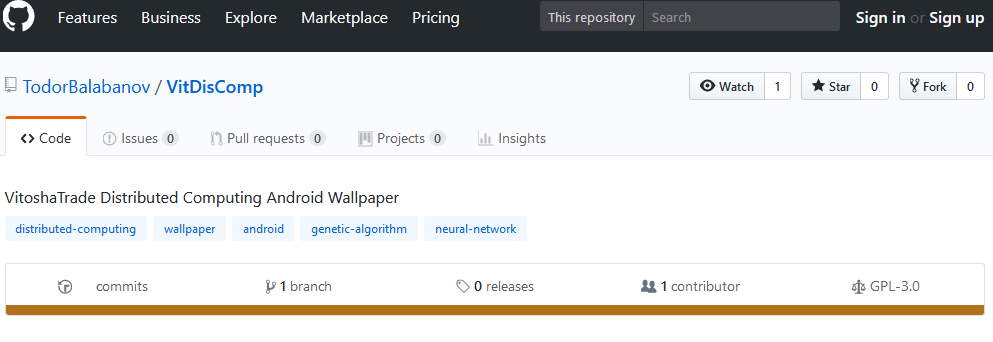
\includegraphics[width=1.0\linewidth]{pic0010}
  \caption{Публикуване на проект в GitHub}
\label{fig:pic0010}
\end{figure}

Съществуват различни възможности за публикуване на програмния код, но една от най-популярните алтернативи е облачната услуга GitHub. Услугата GitHub (Фиг. \ref{fig:pic0010}) е базирана на системата за контрол на версиите Git и дава една от най-широките възможности за популяризиране на програмен код с отворен лиценз.